\documentclass{beamer}
%include polycode.fmt
\usepackage{fancyvrb}
\usepackage{qtree}
\usepackage{verbatim}
\usepackage{graphicx}
\usetheme{Warsaw}
%\setbeameroption{show notes}
\title{Caffeine -- The Habit-Forming Compiler}
\author{Justin Bailey}
\date{July 13, 2009}
\begin{document}
%if False
\CustomVerbatimEnvironment{code}{Verbatim}{}
%endif
\VerbatimFootnotes
\DefineShortVerb{\#}

\begin{frame}
\titlepage
\end{frame}

\section{Overview}

\begin{frame}{What is Caffeine?}
  \begin{quote}
    An interpreter and x86 compiler for the Habit language.
  \end{quote}
\end{frame}

\begin{frame}{What is Habit?}
  Habit is \ldots
  \begin{itemize}
  \item Pure
  \item Functional
  \end{itemize}

  And Caffeine says it is \ldots
  \begin{itemize}
  \item Syntactically identical to Haskell
  \item Strict 
  \end{itemize}
\end{frame}

\begin{frame}{What Can Caffeine Do?}
  \begin{itemize}
  \item Parameterized algebraic data types
  \item Higher-order functions, partial application
  \item Pattern-matching, conditionals, case analysis, guards, etc.
  \item Global and local definitions
  \item Mutually recursive definitions (mostly)
  \end{itemize}
\end{frame}

\begin{comment}
  \begin{frame}{Conventions}
    \begin{itemize}
    \item All functions take one argument. 
    \item If present, the @main@ function is the result of the program.
    \end{itemize}
  \end{frame}
\end{comment}

\section{Architecture}

\begin{frame}{Pipeline}
\begin{figure}\centering
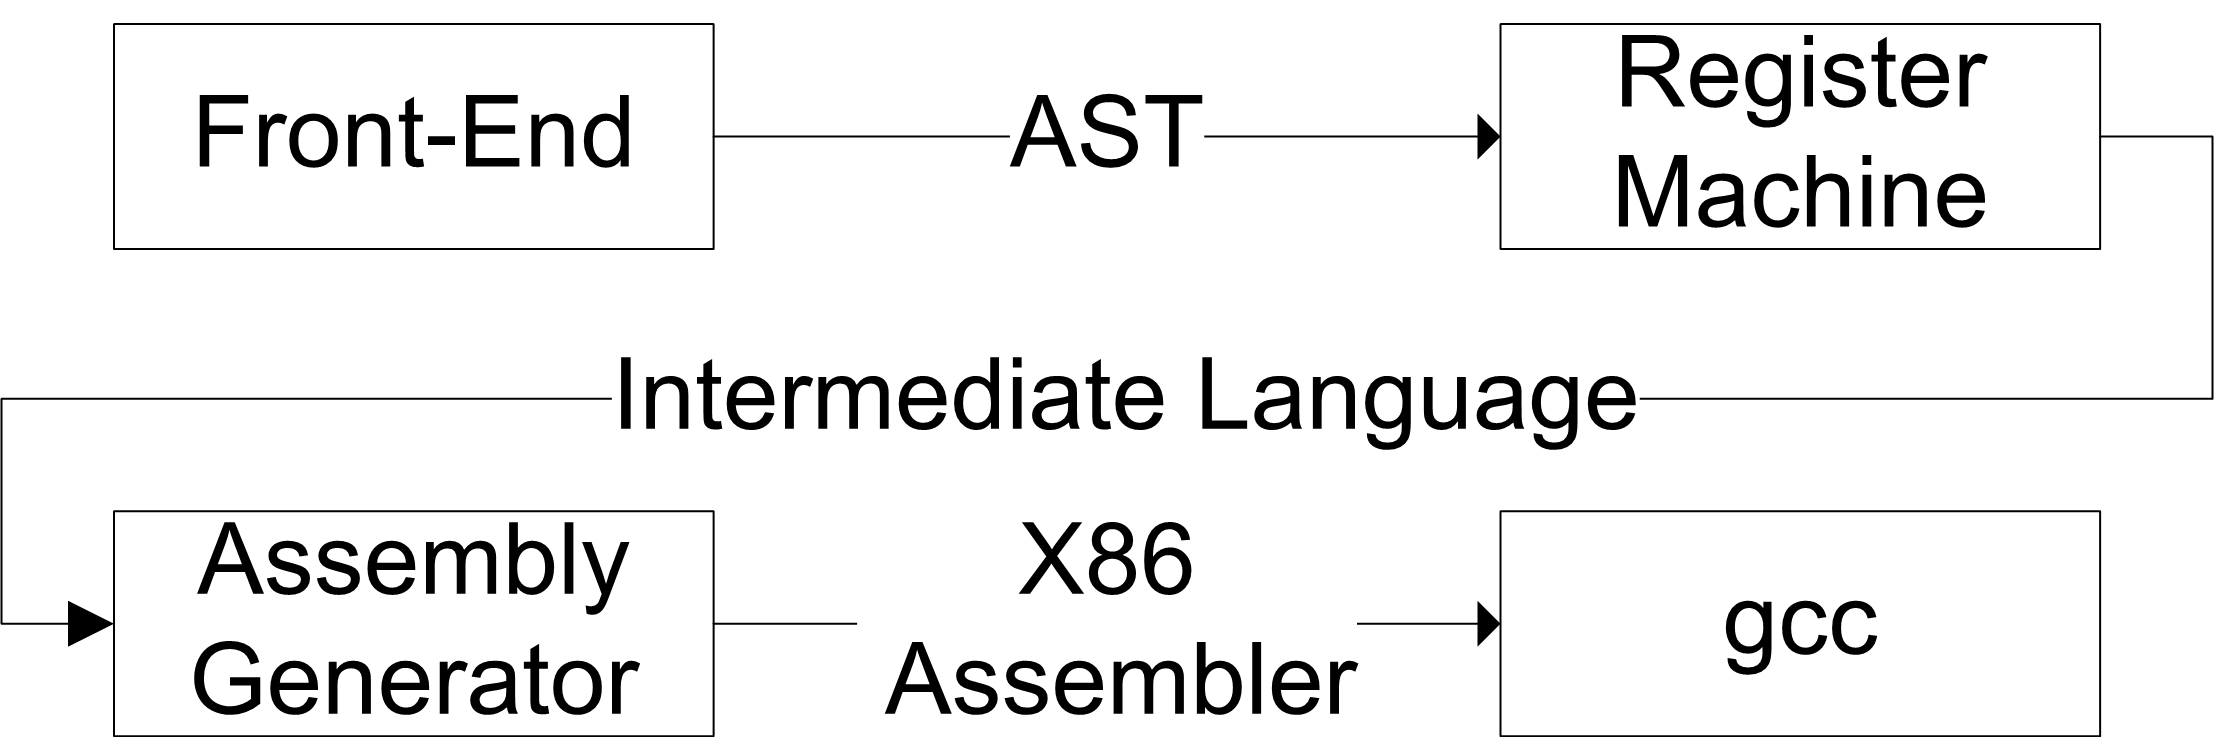
\includegraphics{fig_Pipeline}
\end{figure}
\end{frame}

\begin{frame}[fragile]{Register Machine}
  \begin{itemize}
  \item Runs programs in ``Intermediate Language'' (IL); i.e., an interpreter.
  \item Simple -- easy to map to x86.
  \item Two special registers -- #clo# and #arg#.
  \item IL used as input to x86 compiler.
  \end{itemize}
\end{frame}

\begin{frame}{x86 Compiler}
  \begin{itemize}
  \item Produces x86 assembly from IL source.
  \item Relies on simple runtime for allocation support.
  \item Produces a result by dumping heap value produced by @main@ function.
  \end{itemize}
\end{frame}

\begin{frame}[fragile]{Closures}
  Consider 
\begin{code}
  foldr f a bs
\end{code}

  The front-end gives this AST:

\Tree [.@@
         [.@@
           [.@@
             |foldr|
             |f|
           ]
           |a|
         ]
         |bs|
      ]

\note{Inform audience that Caffeine (and the AST) treat all functions
  as if they took only on argument, which is why three applications
  are present here.}
\end{frame}

\begin{frame}[fragile]{Closures}
  Three applications means three functions:
  \begin{code}
foldr f a bs == ((foldr1 f) a) bs
  \end{code}

  \begin{code}
foldr1 f = foldr2 f
foldr2 f a = foldr f a
foldr f a bs = ...
  \end{code}
\note{foldr f a bs is applied like three separate functions, where each
takes one more argument.}
\end{frame}

\begin{frame}{Closures}
  Register Machine representation:
\begin{figure}\centering

\includegraphics{fig_foldrReg}
\end{figure}

\note{Explain tag/body representation of closures. Use captured
  variables in slots!}
\end{frame}

\begin{frame}{Closures}
  Assembly representation:
\begin{figure}\centering
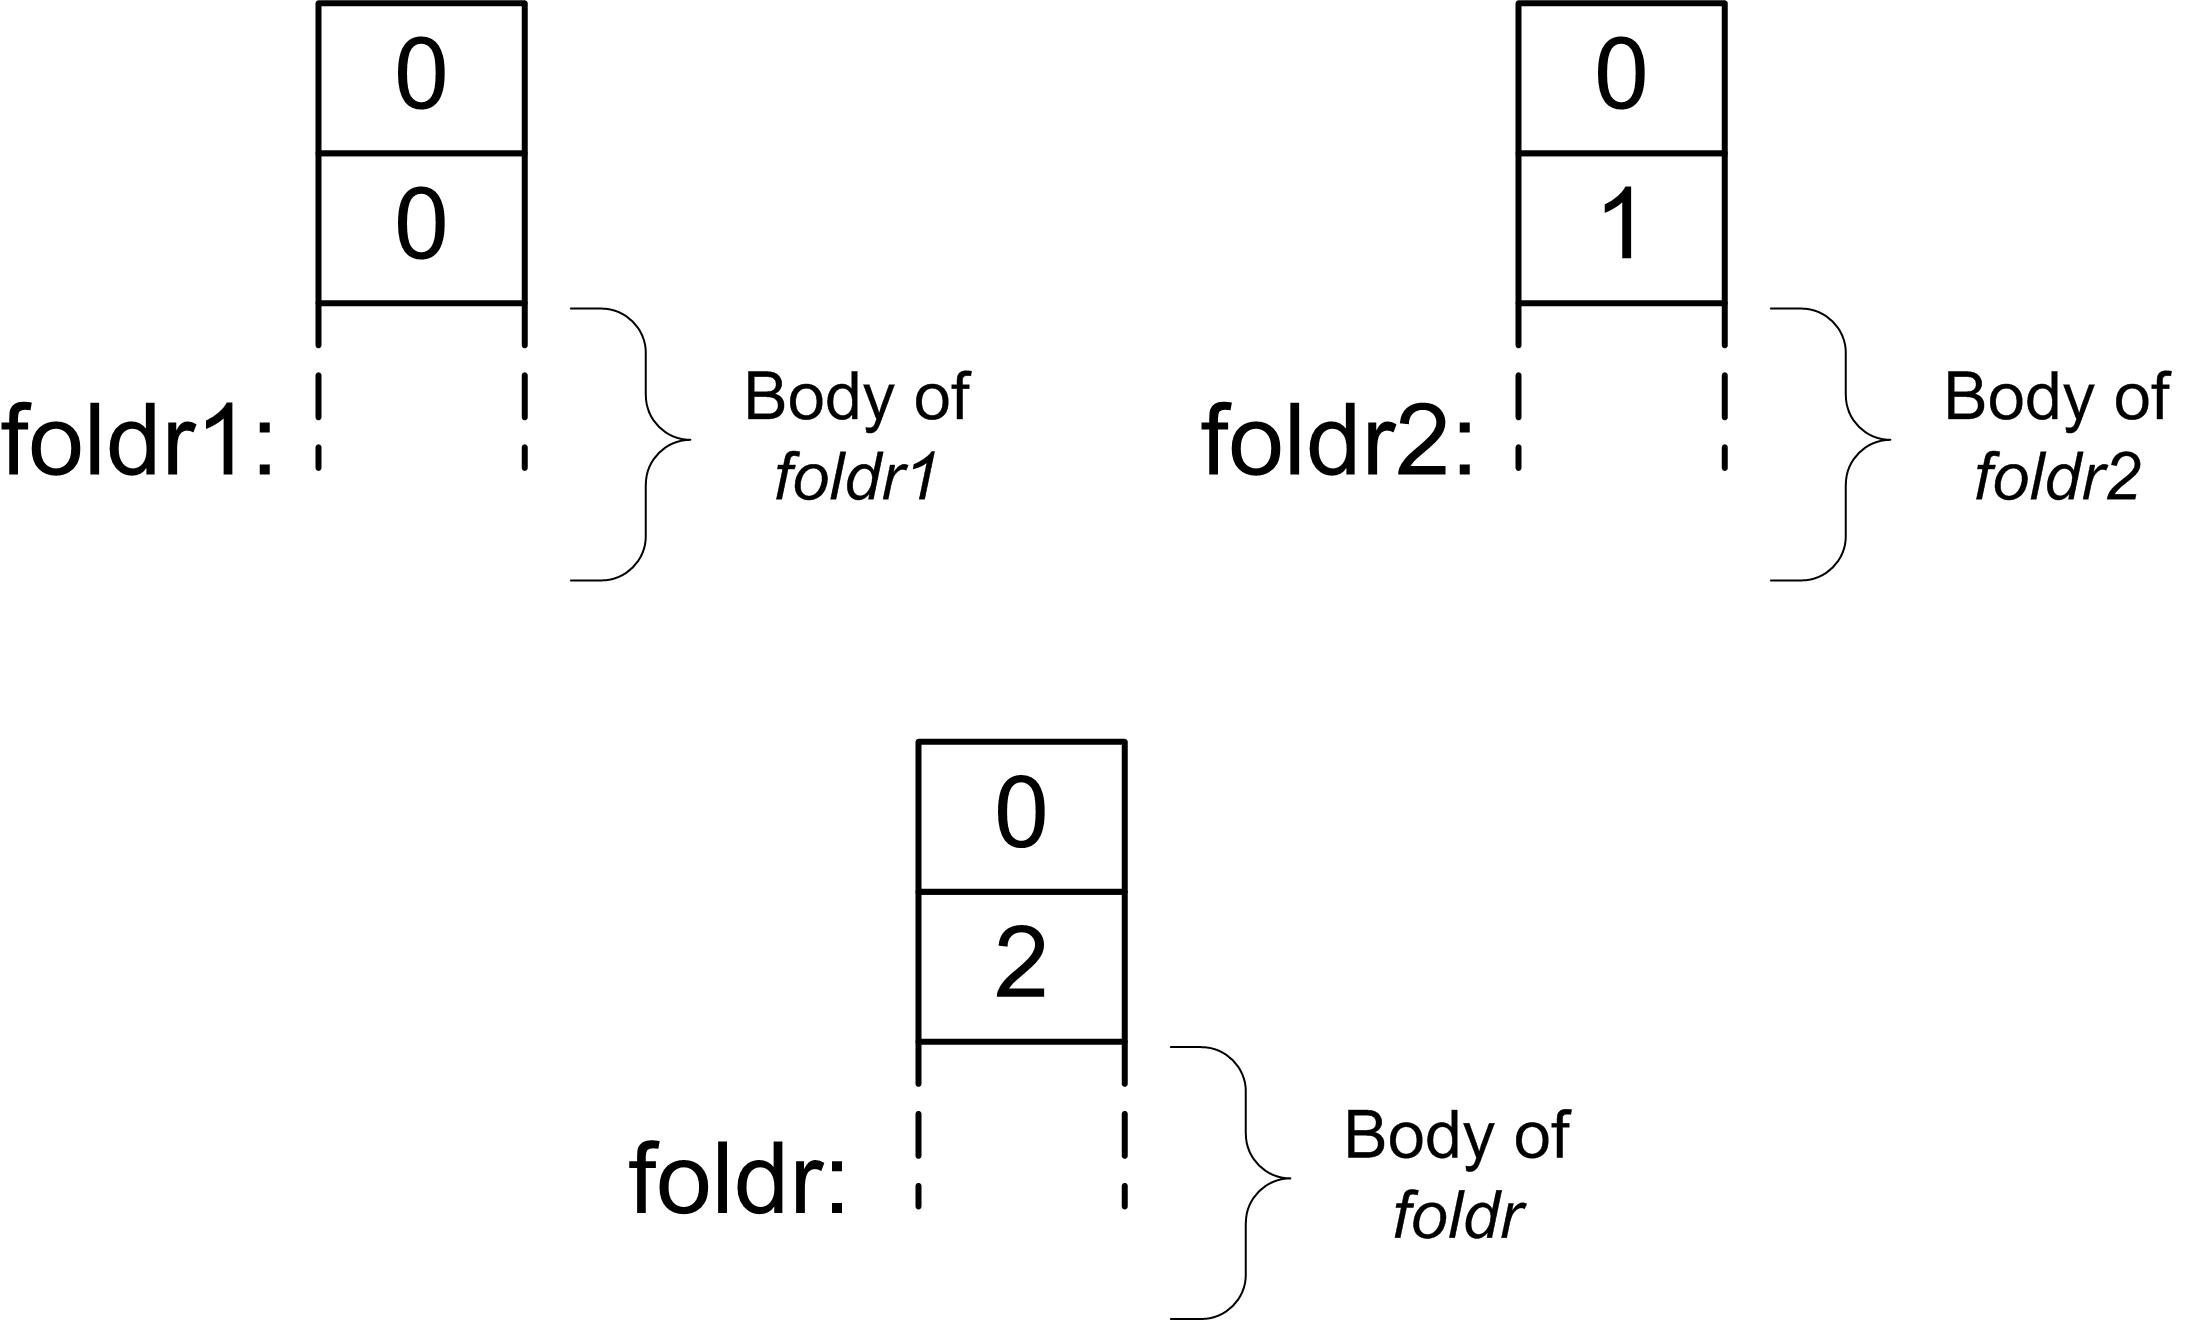
\includegraphics{fig_foldrAsm}
\end{figure}

\note{Show heap layout. Also show info table for at each address. }
\end{frame}

\begin{comment}
  \begin{frame}{Register Machine IL}
    \begin{itemize}
    \item Imperative
    \item First-order
    \item Untyped 
    \item No abstraction facilities (modules, functions, etc.)
    \item Easy translation to x86 assembly.
    \end{itemize}
  \end{frame}
\end{comment}

\begin{frame}[fragile]{|Foldr| in IL}
  |foldr f a bs| in IL. Recall:

\Tree [.@@
         [.@@
           [.@@
             |foldr|
             |f|
           ]
           |a|
         ]
         |bs|
      ]

\note{Emphasize why exploring detail at this level. Want to show
  interaction between closures and application.  Also gives a
  ``flavor'' of what the IL is capable of.}
\end{frame}

\begin{frame}{|Foldr| in IL}
  |Enter| implements application. Top-level evaluation:

  \begin{code}
  Enter foldr1 f result0
  Enter result0 a result1
  Enter result1 bs result2
  \end{code}

  \begin{itemize}
  \item |foldr1| -- Capture |f|.
  \item |result0| -- Capture |a|.
  \item |result1| -- Evalute |foldr| with |bs|.
  \item |result2| -- Result of evaluation of |foldr f a bs|.
  \end{itemize}

\note{Emphasize that each argument to Enter is a register, but for
  clarity labels are shown here.}

\end{frame}

\begin{frame}{|Foldr| in IL}
  |foldr1| captures |f|:

  \begin{code}
  AllocC result0 foldr2 1
  Store arg (result0,0) -- arg special.
  Ret result0
  \end{code}

  |foldr2| copies |f| and captures |a|:
  \begin{code}
  Load (clo,0) f -- clo special.
  AllocC result1 foldr 2
  Store f (result1,0)
  Store arg (result1,1)
  Ret result1
  \end{code}

\note{Briefly explain each instruction, but concentrate on
  AllocC. Note that the second argument is a label/address of a
  function here.}

\end{frame}

\begin{frame}{|Foldr| in IL}
  
  |foldr| is:

  \begin{code}
    foldr f a Nil = a
    foldr f a (Cons b bs) = f b (foldr f a bs)
  \end{code}

Check |Nil| first:
  \begin{code}
  Load (clo,0) f
  Load (clo,1) a
  FailT arg Nil lab28
  ...
  Ret a
  \end{code}

\note{Explain FailT here.}

\end{frame}

\begin{frame}{|Foldr| in IL}
  Next, check |Cons|:
  \begin{code}
lab28: FailT arg Cons lab32
  \end{code}

Evaluate |foldr f a bs| and store in |reg37|.
  \begin{code}
  Load (arg,0) b
  Load (arg,1) bs
  Enter foldr1 f reg35
  Enter reg35 a reg36
  Enter reg36 bs reg37
  \end{code}
\end{frame}

\begin{frame}{|Foldr| in IL}
Finally, evaluate |f a reg37|.
  \begin{code}
  Enter f b reg38
  Enter reg38 reg37 result2
  ...
  Ret result2
  \end{code}
\end{frame}

\begin{frame}{|Foldr| in Assembler}
  Three key instructions from IL to explore
  \begin{itemize}
  \item |Enter| -- Application.
  \item |FailT| -- Conditionals/Discrimination.
  \item |AllocC| -- Allocation.
  \end{itemize}
\note{Don't worry, we aren't going to go into the depth we did on IL!}
\end{frame}

\begin{frame}{|Enter| in Assembler}
  
\begin{verbatim}
    # "Enter foldr1 f result0
    pushl %esi
    pushl %edi
    movl foldr1, %edi
    movl $f, %esi
    call *(%edi)
\end{verbatim}

\note{esi and edi are arg and closure register,
  respectively. foldr1 is the location holding the address of the
  initial closure. f is the address of the function used to fold.}
\end{frame}

\begin{frame}{|FailT| in Assembler}
\begin{verbatim}
    # "FailT arg Nil lab28
    movl (%esi), %ecx
    movl (%ecx), %ecx
    cmpl $0x348, %ecx
    jnz lab28
...
    # "FailT arg Cons lab32
    movl (%esi), %ecx
    movl (%ecx), %ecx
    cmpl $0x3b8, %ecx
    jnz lab32

\end{verbatim}

\note{First move arg into ecx, then dereference ecx to get tag out of
  arg. Compare arg to ``Nil'' and jump to next branch if NOT equal. 

Similarly for Cons.}

\end{frame}

\begin{frame}{|AllocC| in Assembler}
Recall |foldr1| captures |f| and points to |foldr2|:

  \begin{code}
  AllocC result0 foldr2 1
  Store arg (result0,0) -- arg special.
  ...
  \end{code}

In assembler:

\begin{verbatim}
    # AllocC result0 foldr2 1
    pushl $foldr2
    call _alloc
    addl $0x4, %esp
    movl %eax, -4(%ebp)
    # Store arg (result0,0)
    movl %esi, %edx
    movl -4(%ebp), %ecx
    movl %edx, 4(%ecx)
\end{verbatim}

\note{foldr2 is the address of the next function in the application
  chain. -4(ebp) is the location that result0 has been associated
  with.

\_alloc is our runtime function for allocating memory. Implemented in C. }
\end{frame}

\begin{frame}{|AllocC| in Assembler}
Preceding \verb_$foldr2_ we find the \emph{info table} for the closure:
\begin{verbatim}
    .long 0x0
    .long 0x1
foldr2:
\end{verbatim}

\note{Explain meaning of entries. Talk about how \_alloc uses this
  information. Perhaps mention that data is allocated in the same
  way?}
\end{frame}

\begin{frame}[fragile]{Composability}

  ``Compiler as Service''

 \note{ Each stage can be independently executed with the outputs from
   the previous stage.

 Output of each stage can persisted and re-used later.  

 Composable pipeline of stages.}
\end{frame}

\begin{frame}[fragile]{Composable Signatures}
  \begin{itemize}
  \item Register Compiler: |Module|/|[Group]|
  \end{itemize}
  
  \begin{code}
   compile :: Supply Int -> Module -> [Group]
  \end{code}
  
\begin{itemize}
  \item Assembly Compiler: |[Group]|/|Program|\footnote[frame]{Dirty secret -- |Program == [String]|.}
  \end{itemize}

  \begin{code}
   assemble :: Supply Int -> [Group] -> Program
 \end{code}

\note{Dirty secret is only temporary!}
\end{frame}

\section{Future Work}
\begin{frame}{What it Does Not Do}
  \begin{itemize}
  \item Primitive types (|Int|, |String|, etc.)
  \item Typeclasses
  \item Input/Output
  \item Multi-module programs
  \item Garbage Collection
  \end{itemize}
\end{frame}

\begin{frame}{What it Could Do}
  \begin{itemize}
  \item All of the above ...
  \item REPL
  \item Debugger
  \item Staged compilation 
  \end{itemize}
\end{frame}

\begin{frame}[fragile]{Where to Find Out More}
  Code available in #cg509#. The #README# will tell you what to do.
\end{frame}

\begin{frame}[fragile]{Samples}
  \begin{itemize}
  \item #tests\Even.hs#
  \item #tests\Fib.hs# 
  \item #tests\Foldr2.hs# 
  \end{itemize}
\end{frame}
\end{document}
